\documentclass[a4paper, 12pt]{article}
\usepackage[T1]{fontenc}
\usepackage[utf8]{inputenc}
\usepackage[french]{babel}
\usepackage{epsfig}
\usepackage{dsfont}
\usepackage{latexsym}
\usepackage{amsmath}
\usepackage{amssymb}
\usepackage{multirow}
\usepackage{color}
\usepackage{mathrsfs}
\usepackage{float} 
\usepackage{bbding}
\usepackage{fancybox}

\usepackage{graphicx}%%%%%%%%%%% standard LaTeX package
                               % for including eps-figure files
                               % or pdf-figure files
\usepackage[titlenotnumbered,ruled,vlined,noend,linesnumbered]{algorithm2e}
\usepackage{array,multirow}

\usepackage[usenames,dvipsnames]{pstricks}
\usepackage{epsfig}
\usepackage{pst-grad} % For gradients
\usepackage{pst-plot} % For axes
 

\newcommand{\bulle}{\textcolor[rgb]{0.00,0.00,1.00}{\bullet}}
\newenvironment{proof}[1][Proof] {\noindent \textcolor[rgb]{0.00,0.00,1.00}{\textbf{#1:}} \\ } {\ \textcolor[rgb]{0.00,0.00,1.00}{\textbf{\rule{0.5em}{0.5em}}} \bigskip}
\newcommand{\R}{\mathbb{R}}
\newcommand{\N}{\mathbb{N}}
\newcommand{\E}{\mathbb{E}}
\newcommand{\D}{\mathbb{D}}
\newcommand{\cov}{\text{cov}}
\newcommand{\cor}{\text{cor}}
\newcommand{\cog}{\text{cog}}
\newcommand{\y}{\mathbf{y}}
\newcommand{\Step}{\underline{\textbf{Step}}}
\newcommand{\eps}{\varepsilon}
\newcommand{\z}{\mathbf{z}}
\newtheorem{resultat}{Résultat}
\newtheorem{condition}{Condition}
\newtheorem{proposition}{Proposition}
\newtheorem{property}{Property}
\newtheorem{conjecture}{Conjecture}
\newtheorem{corollary}{Corollary}
\newtheorem{criterion}{Criterion}
\newtheorem{stat}{Statement}
\newtheorem{axiom}{Axiom}
\newtheorem{definition}{Definition}
\newtheorem{example}{Example}
\newtheorem{lemma}{Lemma}
\newtheorem{remark}{Remarque}
\newtheorem{theorem}{Theorem}
%\input{tcilatex}
\numberwithin{equation}{section}



\begin{document}

\section{L'opérateur Gini covariance}

Soit $\bar{x}_k$ la moyenne arithmétique de la variable $x_k$. L'opérateur de Gini covariance proposé par Schechtman and Yitzhaki (1987), encore appelé opérateur co-Gini est donné par:
\begin{equation}\label{cog0}
\cog(x_\ell,x_k) := \cov(x_\ell,F(x_k)) = \frac{1}{N}\sum_{i=1}^N(x_{i\ell} -\bar{x_\ell})(\hat{F}(x_{ik})-\bar{F}_{x_k}),
\end{equation}
où $\hat{F}(x_{k})$ est la fonction de répartition de $x_k$, $\bar{F}_{x_k}$ sa moyenne, avec $\ell \neq k = 1,\ldots,K$. Lorsque $k=\ell$ le co-Gini mesure la variabilité entre une variable et elle-même (l'équivalent de la variance mesurée sur la norme $\ell_2)$. Le co-Gini est une mesure basée sur la distance de Manhattan (distance de métrique $\ell_1$), en effet :
\begin{equation}\notag
\frac{1}{N^2}\sum_{i=1}^N\sum_{j=1}^N |x_{ik} - x_{jk}| = 4\cog(x_k,x_k).
\end{equation}
D'autre part, lorsque $k\neq \ell$, le co-Gini produit une mesure de la variabilité jointe entre deux variables. Puisque le co-Gini n'est pas symétrique :
\[
\cog(x_k,x_\ell) := \cov(x_k ,F(x_\ell)) = \frac{1}{N}\sum_{i=1}^N(x_{ik} -\bar{x_k})(\hat{F}(x_{i\ell})-\bar{F}_{x_\ell}).
\]
Définissons les rangs croissants d'une variable alétoire afin de fournir un estimateur de $F$,
\[
R_\uparrow(x_{i\ell}) := N\hat{F}(x_{i\ell)} = 
\left\{ \begin{array}{ll}
\#\{ x \leq x_{i\ell} \} & \text{si aucune observation similaire} \\
\frac{\sum_{i=1}^p\#\{ x \leq x_{i\ell}  \}}{p} & \text{s'il existe $p$ valeurs similaires $x_{i\ell}$.}
\end{array}
\right.
\]
Alors, un estimateur du co-Gini est donné par,
\begin{eqnarray}\label{cog}
\widehat{\cog}(x_\ell,x_k) := \frac{1}{N}\sum_{i=1}^N(x_{i\ell} -\bar{x_\ell})(R_\uparrow(x_{ik})-\bar{R_\uparrow}_{x_k}), \ \forall k,\ell=1,\ldots,K,
\end{eqnarray}
avec $\bar{R_\uparrow}_{x_k}$ la moyenne arithmétique du vecteur rang de la variable $x_k$. 


\section{Gini-PLS}
 
Le premier algorithme Gini-PLS a été proposé par Mussard et Souissi-Benrejab (2018). Nous le décrivons dans les lignes qui suivent. Il s'agit d'une méthode de compression avec débruitage qui consiste à réduire les dimensions de l'espace généré par $X$ afin de trouver des composantes principales débruitées, dans le même esprit qu'une ACP débruitée, néanmoins l'approche est supervisée dans la mesure où une variable cible $y$ est prise en compte dans le changement d'espace. Le sous-espace formé par les composantes principales $\{t_1,t_2,\cdots\}$ est construit de telle sorte que le lien entre les variables explicatives $X = [x_1,x_2,\cdots]$ et la cible $y$ est maximisé.  \textcolor{red}{$\vert X \vert = p$, nombre de variables explictives}.

\medskip

$\bulle$ \underline{\textbf{Étape 1:}} La régression Gini permet de concevoir un nouveau type de lien entre la variable expliquée et les variables explicatives tout en évitant l'influence des valeurs aberrantes. Ceci est permis grâce notamment à l'opérateur co-Gini dans lequel le rôle de la variable explicative est remplacé par celui de son vecteur rang dans un espace muni d'une métrique $\ell_1$.  Ainsi, il est possible de créer un nouveau vecteur de poids $w_1$ qui renforce le lien (co-Gini) entre la variable expliquée $y$ et les régresseurs $X$ dans le cadre d'une régression (linéaire ou non linéaire).
\newline La solution du programme,
\[
\max \cog(y,X w_1) \ , \ \text{s.c.} \ \left\|w_1\right\|=1 \ , \ \text{est}
\]
\begin{equation}\notag
w_{1j} = \frac{\cog(y,x_j)}{\sqrt{\sum_{j=1}^p \emph{cog}^2(y,x_j)}} \ , \ \forall j = 1\ldots,p \ .
\end{equation}
La pondération est équivalente à :
\begin{equation}\notag
w_{1j} = \frac{\cov(y,R(x_j))}{\sqrt{\sum_{j=1}^p \cov^2(y,R(x_j))}} \ , \ \forall j = 1\ldots,p \ .
\end{equation}
Comme dans la régression PLS, on régresse $y$ sur la composante $t_1$ qui est construite de la manière suivante :
\[
t_1 = \sum_{j=1}^p w_{1j}x_j \ \Longrightarrow \ y = \hat{c}_1 t_1 + \hat{\varepsilon}_1 \ .
\]

\medskip

$\bulle$ \underline{\textbf{Étape 2:}}  On régresse le vecteur rang de chaque régreseur $R(x_j)$ sur la composante $t_1$ par moindres carrés ordinaires afin de récupérer les résidus $\hat{U}_{(1)j}$ : 
\[
R(x_j) = \hat{\beta}t_1 + \hat{U}_{(1)j} \ , \ \forall j = 1,\cdots, p \ .
\]
On construit le nouveau vecteur de pondération en utilisant les rangs des résidus des régressions partielles :
\[
\max \text{cog}(\hat{\varepsilon}_1,\hat{U}_{(1)} w_2) \ , \ \text{s.c.} \ \left\|w_2\right\|=1 \ \Longrightarrow \ w_{2j} = \frac{\cog(\hat{\varepsilon}_1,\hat{U}_{(1)j})}{\sqrt{\sum_{j=1}^p \cog^2(\hat{\varepsilon}_1,\hat{U}_{(1)j})}} .
\]
On utilise à présent les composantes $t_1$ et $t_2$ pour établir un lien entre $y$ et les régresseurs $x_j$ :
\[
t_2 = \sum^p_{j=1} w_{2j} \hat{U}_{(1)j} \ \Longrightarrow \ y = \hat{c}_1 t_1 + \hat{c}_2 t_2 + \hat{\varepsilon}_2 \ .
\]
La validation croisée permet de savoir si $t_2$ est significative.\\

$\bulle$ \underline{\textbf{Étape 3:}} Les régressions partielles sont réitérées en rajoutant l'influence de $t_2$ :
\[
R(x_j) = \beta t_1 + \gamma t_2 + \hat{U}_{(2)j} \ , \ \forall j = 1,\cdots, p.
\]
D'où, après maximisation :
\[
w_{3j} = \frac{\cog(\hat{\varepsilon}_2,\hat{U}_{(2)j})}{\sqrt{\sum_{j=1}^p \cog^2(\hat{\varepsilon}_2,\hat{U}_{(2)j})}} \ ,
\]
\[
t_3 = \sum_{j=1}^p w_{3j}\cdot \hat{U}_{(2)j} \ \Longrightarrow \ y = \alpha_2 + c_1 t_1 + c_2 t_2 + c_3 t_3 + \varepsilon_3 \ .
\]
La procédure s'arrête lorsque la validation croisée indique que la composante $t_l$ n'est pas significative. L'algorithme Gini-PLS1 est valable si toutes les composantes $t_h$ et $t_l$ sont orthogonales, $\forall h\neq l$. 

\medskip

La validation croisée permet de trouver le nombre optimal $h>1$ de composantes à retenir. Pour tester une composante $t_h$, on calcule la prédiction du modèle avec $h$ composantes comprenant l'observation $i$, $\hat{y}_{h_i}$, puis sans l'observation $i$, $\hat{y}_{h_{(-i)}}$. L'opération est répétée pour tout $i$ variant de $1$ à $n$ : on enlève à chaque fois l'observation $i$ et on ré-estime le modèle.\footnote{Les observations peuvent être éliminées bloc par bloc au lieu de l'être une à une, \emph{Cf.} Tenenhaus (1998), p. 77.} Pour mesurer la robustesse du modèle, on mesure l'écart entre la variable prédite et la variable observée :
\[
PRESS_h =  \sum_i\left(y_i - \hat{y}_{h_{(-i)}}\right)^2 \ .
\]
La somme des carrés résiduels obtenue avec le modèle à $(h-1)$ composantes est : 
\[
RSS_{h-1} = \sum \left(y_i - \hat{y}_{(h-1)_i}\right)^2 \ .
\]
Le critère $RSS_h$ (Residual Sum of Squares) du modèle à $h$ composante et $PRESS_h$ (PRedicted Error Sum of Squares) sont comparés. Leur ratio permet afin de savoir si le modèle avec la composante $t_h$ améliore la prédictibilité du modèle. La statistique suivante est alors calculée :
\[
Q^2_h =1 - \frac{PRESS_h}{RSS_{h-1}} \ .
\]
La composante $t_h$ est retenue si : $\sqrt{PRESS_h} \leq 0,95 \sqrt{RSS_h}$. Autrement dit, lorsque $Q^2_h \geq 0,0975 = (1 - 0,95^2)$, la nouvelle composante $t_h$ est significative, elle améliore la prévision de la variable $y$. Pour la significativité de de la première composante $t_1$,  on utilise :
\[
RSS_0 = \sum^{n}_{i = 1} \left(y_i - \bar{y}\right)^2  \ .
\]


\section{Propositions : régressions Gini-PLS généralisée} 

Schechtman and Yitzhaki (2003) ont récemment généralisé l'opérateur co-Gini afin d'imposer plus ou moins de poids en queue de distribution. Notons $r_{k}=(R_\downarrow(x_{1k}),\ldots, R_\downarrow(x_{Nk}))$ le vecteur rang décroissant de la variable $x_k$, autrement dit, le vecteur qui assigne le rang le plus petit (1) à l'observation dont la valeur est la plus importante (et positive) $x_{ik}$ :
\[
R_\downarrow(x_{ik}) :=
\left\{ \begin{array}{ll}
N+1- \#\{x \leq x_{ik} \} & \text{pas d'observation similaire} \\
N+1-\frac{\sum_{i=1}^p \#\{ x \leq x_{ik}  \}}{p} & \text{si $p$ observations similaires $x_{ik}$.}
\end{array}
\right.
\]
L'opérateur co-Gini est généralisé grâce au paramètre $\nu$ :
\begin{equation}\label{cogg}
\widehat{\cog}_\nu(x_\ell,x_k) := -\nu \widehat{\cov}(x_\ell,r_{k}^{\nu-1}) ;  \ \nu > 1.
\end{equation}
Afin de bien comprendre le rôle de l'opérateur co-Gini, revenons sur la mesure du coefficient de corrélation linéaire généralisé au sens de Gini :
\[
GC_\nu(x_\ell,x_k) := \frac{-\nu \widehat{\cov}(x_\ell,r_{k}^{\nu-1})}{-\nu \widehat{\cov}(x_\ell,r_{\ell}^{\nu-1})} \ ; \ GC_\nu(x_k,x_\ell) := \frac{-\nu \widehat{\cov}(x_k,r_{\ell}^{\nu-1})}{-\nu \widehat{\cov}(x_k,r_{k}^{\nu-1})}.
\]

\begin{property}\label{prop1} -- \textbf{\emph{Schechtman et Yitzhaki (2003):}}

\noindent \emph{(i)} $GC_\nu(x_\ell,x_k) \leq 1$.

\noindent\emph{(ii)} Si les variables $x_\ell$ et $x_k$ sont indépendantes, pour tout $k\neq \ell$, alors $GC_\nu(x_\ell,x_k) = GC_\nu(x_k,x_\ell) =0$.

\noindent\emph{(iii)} Une transformation monotone des données $\varphi$ n'affecte pas le coefficient de corrélation, $GC_\nu(x_\ell,\varphi(x_k)) = GC_\nu(x_\ell,x_k)$.

\noindent\emph{(iv)} Pour une transformation linéaire $\varphi$, $GC_\nu(\varphi(x_\ell),x_k) = GC_\nu(x_\ell,x_k)$ $[$comme le coefficient de corrélation de Pearson$]$.

\noindent\emph{(v)} Si $x_k$ et $x_\ell$ sont deux variables échangeables à une transformation linéaire près, alors $GC_\nu(x_\ell,x_k) = GC_\nu(x_k,x_\ell)$.
\end{property}

Le rôle de l'opérateur co-Gini peut être expliqué de la manière suivante. Lorsque $\nu \rightarrow 1$, la variabilité des variables est atténuée de telle sorte que $\cog_\nu(x_k,x_\ell)$ tend vers zéro (même si les variables $x_k$ et $x_\ell$ sont fortement corrélées).Au contraire, si $\nu \rightarrow \infty $ alors $\cog_\nu(x_k,x_\ell)$ permet de se focaliser sur les queues de distribution $x_\ell$. Comme le montrent Olkin and Yitzhaki (1992), l'emploi de l'opérateur co-Gini atténue la présence de valeurs extrêmes, du fait que le vecteur rang agit comme un instrument dans la régression de $y$ sur $X$ (régression par variables instrumentales).    

Ainsi, en proposant une régression Gini-PLS basée sur le paramètre $\nu$, nous pouvons calibrer la puissance du débruitage  grâce à l'opérateur co-Gini qui va localiser le bruit dans la distribution. Cette régression Gini-PLS généralisée devient une régression Gini-PLS régularisée où le paramètre $\nu$ joue le rôle de paramètre de régularisation. 


\subsection{L'algorithme Gini-PLS généralisé} 

Dans ce qui suit nous généralisons la régression Gini-PLS de Mussard et Souissi-Benrejab (2018) avec renforcement du pouvoir de débruitage par l'intermédiaire du paramètre $nu$.


\begin{center}
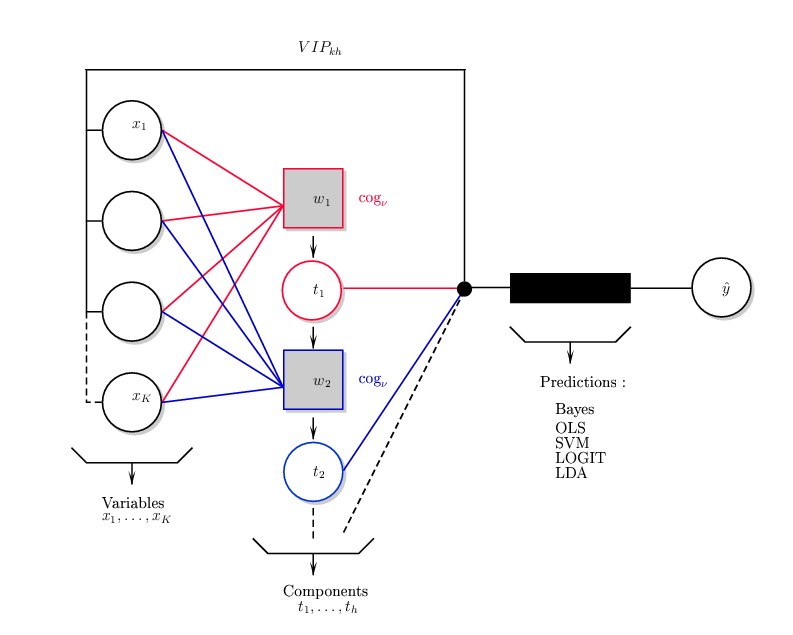
\includegraphics[scale=0.5]{graph.png}
\end{center}


La première étape consiste à trouver des poids de débruitage associés à chaque variable $x_k$ afin d'en déduire la première composante $t_1$ (ou première variable latente). Cette opération est bouclée jusqu'à la composante $t_{h^*}$, où $h^*$ est le nombre optimal de variable latentes. Ainsi, le modèle est estimé :
\begin{equation}\label{forecast}
y=\sum_{h=1}^{h^*} c_ht_h +\eps_h.
\end{equation}   
La statistique $VIP_{hj}$ est mesurée afin de sélectionner la variable $x_j$ qui a l'impact significatif le plus important sur $\hat{y}$. Les variables les plus significatives sont celles dont $VIP_{hj}>1$ avec :
\[
VIP_{hj} := \sqrt{\frac{p\sum_{\ell=1}^{h}Rd(y;t_\ell)w_{\ell j}^2}{Rd(y;t_1,\ldots,t_h)}} 
\] 
et 
\[
Rd(y; t_1,\ldots,t_h) := \frac{1}{p}\sum_{\ell=1}^{h}\cor^2(y,t_\ell) =: \sum_{\ell=1}^{h}Rd(y;t_\ell).
\]
où $cor^2(y,t_\ell)$ est le coefficient de corrélation de Pearson entre $y$ et la composante $t_\ell$. Cette information est rétro-propagée dans le modèle (une seule fois) afin d'obtenir les variables latentes $t_{h^*}$ et leurs coefficients estimés $\hat{c}_{h^*}$ sur les données d'entrainement. La variable cible $y$ est ensuite prédite grâce à (\ref{forecast}). Cette prévision est comparée aux modèles standards SVM, LOGIT, Bayes et LDA lorsque les données tests sont projetées dans le sous-espace $\{t_1,\ldots,t_{h^*}\}$.\\


\begin{algorithm}[H]
\KwResult{ Prédiction du juge $y=0;1$ }
	\Repeat{ $\nu=14$ $[\nu=\nu+2]$ }{
	\Repeat{ $h=10$ $[h=h+1]$ }{
$\max \cog_\nu(y,w_hX)$ s.t. $\| w_h\|=1$ $\Longrightarrow$ poids $w_h$ de $X$ \;
MCO équation: $y=\sum_h c_ht_h +\eps_h$ \;
MCO équation: $R(x_j)=\sum_h \beta_ht_h + \epsilon_k$ $\forall k=1,\ldots,K$ \;
$X:=(\hat{\epsilon}_1,\ldots,\hat{\epsilon}_K)$ $y:=\hat{\eps}_h$ \; }
Mesurer $VIP_{kh}$, $Q^2_h$ \;
Sélectionner le nombre optimal de composantes $h^*$ \; }
Déduire le paramètre optimal $\nu^*$ qui minimise l'erreur \; 
\Return Prédiction $\hat{y}$ avec Gini-PLS ($h^*$, $\nu^*$) \;
\Return Prédiction $\hat{y}$ avec SVM, LOGIT, Bayes, LDA sur les composantes $(t_1,\ldots,t_{h^*})$\;
\caption{Gini-PLS Généralisé}\label{G-GPLS}
\end{algorithm}
\bigskip

\subsection{L'algorithme LOGIT-Gini-PLS généralisé} 

Comme nous le constatons dans l'algorithme Gini-PLS généralisé que nous avons proposé dans le section précédente, les poids $w_j$ proviennent de l'opérateur co-Gini appliqué à une variable booléenne $y=0;1$. Afin de trouver les poids $w_j$ qui maximisent le lien entre les variables $x_j$ et la variable cible $y$, nous proposons d'utiliser la régression LOGIT, autrement dit, une sigmoïde qui est bien adapté à des variables boléennes. Ainsi, dans chaque étape de la régression Gini-PLS nous remplaçons la maximisation du co-Gini par la mesure de la probabilité conditionnelle suivante :
\begin{equation}\tag{LOGIT}
\mathbb{P}(y_i = 1 / X = X_i) = \frac{\exp\left\{X_i \beta \right\}}{1+\exp\left\{ X_i \beta \right\}}
\end{equation}
où $X_i$ est la ième ligne de la matrice $X$ (observation des caractéristiques/dimensions de la décision juridique $i$). L'estimation du vecteur $\beta$ se fait maximum de vraisemblance. On en déduit alors les pondérations $w_j$ :
\[
w_j = \frac{\beta_j}{\| \beta\|}
\]
L'algorithme LOGIT-Gini-PLS généralise est donc le suivant :

\begin{algorithm}[H]
\KwResult{ Prédiction du juge $y=0;1$ }
	\Repeat{ $\nu=14$ $[\nu=\nu+2]$ }{
	\Repeat{ $h=10$ $[h=h+1]$ }{
LOGIT équation : $\Longrightarrow$ poids $w_j$ de $X$ \;
MCO équation : $y=\sum_h c_ht_h +\eps_h$ \;
$X:=(\hat{\epsilon}_1,\ldots,\hat{\epsilon}_K)$ $y:=\hat{\eps}_h$ \; }
Mesurer $VIP_{kh}$, $Q^2_h$ \;
Sélectionner le nombre optimal de composantes $h^*$ \; }
Déduire le paramètre optimal $\nu^*$ qui minimise l'erreur \; 
\Return Prédiction $\hat{y}$ avec Gini-PLS ($h^*$, $\nu^*$) \;
\Return Prédiction $\hat{y}$ avec SVM, LOGIT, Bayes, LDA sur les composantes $(t_1,\ldots,t_{h^*})$\;
\caption{LOGIT-Gini-PLS Généralisé}\label{G-GPLS}
\end{algorithm}
\bigskip


\begin{thebibliography}{18}

\bibitem{SM} Mussard, S. and F. Souissi-Benrejab (2018), Gini-PLS regressions, \emph{Journal of Quantitative Economics}, 1-36, https://doi.org/10.1007/s40953-018-0132-9.

\bibitem{Schechtman03} Schechtman, E., Yitzhaki, S. (2003). A family of correlation coefficients based on extended Gini, \emph{Journal of Economic Inequality}, 1, 129--146. 

\bibitem{wold} Wold, S., Martens, H., Wold, H. (1983). The multivariate calibration problem in chemistry solved by the PLS method, in \textit{Proc. Conf. Matrix Pencils}, Rnhe, A., and Kagstroem, B. (eds), Springer-Verlag: Berlin.  pp. 286--293.

\bibitem{Yitzhaki12} Yitzhaki, S., Schechtman, E. (2013). \emph{The Gini Methodology: A Primer on a Statistical Methodology}, Springer-Verlag: Berlin.

\end{thebibliography} 
\end{document}